\chapter{Ley de acción de masas}

Ahora dejamos los puentes y cambiamos a otro tipo de modelos totalmente diferentes. Vamos a hablar de la ley de acción de masas, pero primero vamos a repasar un poco algunas nociones sobre reacciones químicas. Tenemos una serie de productos $A_1,\cdots, A_n$, $B_1,\cdots, B_n$ y una serie de coeficientes que nos indican la concentración de cada producto: $\alpha_1,\cdots, \alpha_n$, $\beta_1,\cdots, \beta_n$. A estos coeficientes se les llama \textit{coeficientes estequiométricos}. Estos elementos nos dan una reacción química, que expresaremos como:
\[
\alpha_1A_1+\cdots+\alpha_nA_n \longrightarrow \beta_1B_1+\cdots+\beta_nB_n
\]
\begin{example} La reacción química de la quema de hidrógeno:
\[
2H_2+0_2\longrightarrow 2H_20
\]
Otra diferente:
\[
ClH+NaOH \longrightarrow ClNa+H_20
\]
\end{example}

Esto es una cuestión molecular y trabajar con ellas es bastante complicado. Para solventar ese problema, usamos los \textit{moles}. Un \textit{mol} es la cantidad de una sustancia que contiene tantos átomos como su peso atómico. También usaremos la \textit{concentración de un producto}, $[N]$, que es el igual al número de moles que hay del producto. En la reacción anterior obtendríamos dos moles de agua, combinando dos moles de hidrógeno y un mol de oxígeno. Podemos hablar de concentración de \textit{reactivos} y \textit{productos}: $[A] = \{ \text{ número de moles de reactivo } \}$, $[B] = \{ \text{ número de moles de producto } \}$

Por otro lado, está la denominada \textit{velocidad de reacción}, que es la variación de la concentración a lo largo del tiempo. La teoría nos dice que:
\[
\frac{d}{dt}[B]=k[A_1]\cdots[A_n]
\]
\begin{example}
Sean $X,Y$ y $Z$ tre compuestos químicos que se combinan en un producto final $F$ según la reacción:
\[
2X+3Y+5Z\longrightarrow 5F
\]
La velocidad de reacción (moléculas más o menos iguales) se puede suponer proporcional al producto de concentraciones de productos $X,Y,Z$, según un coeficiente $\beta$ (velocidad de reacción). Suponemos que $\beta=0.01$. Si partimos inicalmente de 5 moles de $X$, 7 moles de $Y$ y 10 moles de $Z$, plantear un modelo que permita calcular la concentración de cada sustancia en cada instante. ¿Qué pasará tras mucho tiempo?

Básicamente hay que aplicar una regla de 3:
\[
\left.
\begin{array}{ccc}
2X & \longrightarrow & 5F\\
5X & \longrightarrow & ?
\end{array}
\right\} \Rightarrow \text{ se producirían  12.5F}
\]
\[
\left.
\begin{array}{ccc}
3Y & \longrightarrow & 5F\\
7Y & \longrightarrow & ? = 
\end{array}
\right\} \Rightarrow \text{ se producirían  11.6F }
\]
\[
\left.
\begin{array}{ccc}
5Z & \longrightarrow & 5F\\
10Z & \longrightarrow & ? = 10 
\end{array}
\right\} \Rightarrow \text{ se producirían  10F }
\]
De aquí, deduzco que se van a producir 10 moles de $F$, ya que es el mínimo de las 3 reglas que hemos hecho. Ahora tenemos que ver cuanta cantidad queda de los reactivas $X$ e $Y$ al crear 10 moles de $F$.
\[
\left.
\begin{array}{ccc}
2X & \longrightarrow & 5F\\
? & \longrightarrow & 10F
\end{array} 
\right\}
\Rightarrow \text{ se gastan 4X }
\]
\[
\left.
\begin{array}{ccc}
3Y & \longrightarrow & 5F\\
? & \longrightarrow & 10F
\end{array}
\right\} \Rightarrow \text{ se gastan 6Y }
\]
Luego sobran 1 de $X$, 1 de $Y$ y 0 de $Z$, y se habrán creado 10 moles de $F$. Ahora vamos a denotar por $x(t),y(t),z(t),F(t)$ a la concentración de $X,Y,Z,F$ en el instante $t$ respectivamente. En el instante $t=0$, tendremos las concentraciones iniciales, y en el instante $t=1$, tendremos las finales (el resultado de las cuentas que hemos hecho antes), es decir:
\[
\begin{array}{|c|c|c|}
\hline
& t=0 & t=1 \\
\hline
x(t) & 4 & 1\\
\hline
y(t) & 7 & 1\\
\hline
z(t) & 10 & 1\\
\hline
F(t) & 0 & 1\\
\hline
\end{array}
\]
Si nos fijamos, $5-x(t),7-y(t),10-z(t)$ son los restantes de los productos $X,Y,Z$ en el instante $t$. Es decir, tenemos que la velocidad de reacción de $F$ es:
\[
F'(t)=\beta x(t)y(t)z(t)
\]
Haciendo otra regla de 3:
\[
\left.
\begin{array}{ccc}
2X & \longrightarrow & 5F\\
5-x(t) & \longrightarrow & F(t)
\end{array}
\right\} \Rightarrow F(t)=\frac{5(5-x(t))}{2} \Rightarrow x(t)=5-\frac{2F(t)}{5}
\]
De forma análoga, obtenemos las expresiones de $y(t)$ y $z(t)$:
\[
y(t)=7-\frac{3F(t)}{5}, \espacio z(t)=10-F(t)
\]
Es decir, la expresión final de la velocidad de reacción sería:
\[
F'(t)=0.01\left(5-\frac{2F(t)}{5}\right)\left(7-\frac{3F(t)}{5}\right)\left(10-F(t)\right), \espacio F(0)=0
\]

Si llamamos $g(F)=0.01\left(5-\frac{2F}{5}\right)\left(7-\frac{3F}{5}\right)\left(10-F\right)$, que tiene raíces $F=10,35/3,12.5$. 

\begin{center}
\begin{tikzpicture}[scale=0.5]
\draw (0,0) -- (16,0);
% parabola
\draw[scale=1,domain=0:16,smooth,variable=\x,red] plot ({\x}, {0.01*(5-2*\x/5)*(7-3*\x)*(10-\x)});

% etiquetas
\draw[dashed] (2.3,-0.7) -- (2.3,.2);
\draw (2.3,-1) node[anchor=north] {$10$};
\draw[dashed] (10,-0.7) -- (10,.2);
\draw (10,-1) node[anchor=north] {$\frac{35}{3}$};
\draw[dashed] (12.7,-0.7) -- (12.7,.2);
\draw (12.7,-1) node[anchor=north] {$12.5$};

\draw (2,2) node[] {$g(F)$};

\end{tikzpicture}
\end{center}

Ahora vamos a abstraer un poco el problema para no tener que trabajar con todos los números particulares. Supongamos que tenemos el problema de valores iniciales:
\[
\left\{
\begin{array}{l}
x'=g(x) \\
x(0)=x_0, \espacio x_0<\alpha_1
\end{array}
\right.
\]
donde $\funcion{g}{\R}{\R}$, $g(\alpha_1)=0$, $g'(\alpha_1)<0$ (para que sea compatible con el dibujo) (\textbf{duda}), $g(x)>0$ si $x\in(-\infty, \alpha_1)$ y $\alpha_1$ es la primera raíz de $g$. 

Como sabemos, el anterior problema de valores iniciales tiene una solución maximal $\funcion{x}{(w_-,w_+)}{\R}$, que además es única. Probemos ahora, una serie de propiedades.
\begin{itemize}
\item $x(t)<\alpha_1, \text{ si } t\in(w_-,w_+)$

Tomamos $t^*\in(w_-,w_+)$ con $x(t^*)=\alpha_1$, entonces $x$ sería solución del problema de valores iniciales:
\[
\left\{
\begin{array}{l}
x'=g(x) \\
x(t^*)=\alpha_1
\end{array}
\right.
\]
cuya solución es la constante, $x(t)=\alpha_1$ $\forall t\in(w_-,w_+)$. (\textbf{duda: no entiendo esta demostracion x'd})

\item $x'(t)>0$ $\forall t\in(w_-,w_+)$

Usando el punto anterior es fácil, ya que $x'(t)=g(x(t))>0$ porque $g(x)$ es positivo para todo $x$ en $(-\infty, \alpha_1)$

\item Necesariamente se tiene que $w_+=+\infty$.

Si $t\in[0,w_+)$, entonces $x_0\leq x(t) < \alpha_1$. Ahora podemos usar la teoría de prolongación de soluciones, que nos dice que si tenemos una solución acotada, podemos prolongarla. $x$ además de estar acotada, está lejos del borde. 

\item $\limitemasinfinito{t}{x(t)}=\alpha_1$

Como $x(t)$ es creciente y acotada, entonces el límite existe, y valdrá $L\in\R$. Evidentemente, $L\leq \alpha_1$. Lo único que tenemos que ver es que $L=\alpha_1$. Para ello, vamos a recordar un resultado general:
\begin{lemma}
Sea $\funcion{x}{(w_-,+\infty)}{\R}\in\mathcal{C}^1$ con $\limitemasinfinito{t}{x(t)}=L\in\R$. Entonces existe una sucesión $t_n\in(w_-,+\infty)$ tal que $t_n\longrightarrow +\infty$, con $x'(t_n)\longrightarrow 0$.
\end{lemma}
\begin{proof}
Considerando la diferencia $x(n+1)-x(n)$ y aplicando el teorema del valor medio, nos queda que:
\[
x(n+1)-x(n)=x'(t_n)(n+1-n)=x'(t_n)
\]
Como $x(n+1)\longrightarrow L \leftarrow x(n)$, $x'(t_n)\longrightarrow 0$.
\end{proof}
Luego al existir el límite anterior, existe también $t_n\longrightarrow +\infty$ tal que $x'(t_n)\longrightarrow 0$, es decir, $g(x(t_n))\longrightarrow 0$.  Pero $g(x(t_n))\longrightarrow g(L)$, luego $L=\alpha_1$, que es la raíz.
\end{itemize}

Como $\alpha_1$ era la primera raíz de $g$, es decir, $\alpha_1=10$, hemos visto que $F(t)\longrightarrow 10$. Pero ojo, simplemente tiende, nunca llegamos a crear los 10 moles enteros, es una asíntota que no se alcanza en tiempo finito. Además $F(t)<10$ $\forall t \in(0,+\infty)$.

Usando la cota sobre $F(t)$ y recordando la expresión de $x(t)$, llegamos a que:
\[
x(t)=5-\frac{2F(t)}{5}>5-4=1 \Rightarrow x(t)\longrightarrow 1
\]
Igual con la $y(t)$ y $z(t)$:
\[
y(t)=7-\frac{3F(t)}{5}>7-6=1 \Rightarrow y(t)\longrightarrow 1
\]
\[
z(t)=10-F(t) \Rightarrow z(t)\longrightarrow 0
\]

Volvemos otra vez a la parte abstracta. Sea $g\in\mathcal{C}^2$ de la forma:

\begin{center}
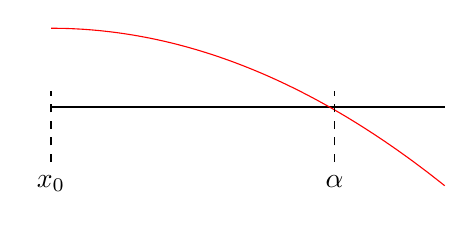
\begin{tikzpicture}
\draw (0,0) -- (5,0);
% parabola
\draw[scale=1,domain=0:5,smooth,variable=\x,red] plot ({\x}, {-0.08*\x*\x+1});

% etiquetas
\draw[dashed] (0,-0.7) -- (0,.2);
\draw (0,-0.75) node[anchor=north] {$x_0$};
\draw[dashed] (3.6,-0.7) -- (3.6,.2);
\draw (3.6,-0.75) node[anchor=north] {$\alpha$};
\end{tikzpicture}
\end{center}

cumpliendo $g(\alpha)=0$ y $g'(\alpha)=\delta<0$. Entonces vamos a tener que (lo que he visto antes):
\[
\limitemasinfinito{t}{x(t)}=\alpha
\]
Ahora vamos a decir un poquito más. Vamos a probar que:
\[
\limitemasinfinito{t}{\frac{x(t)-\alpha}{e^{\delta t}}}=L\in(-\infty,0)
\]
Eso quiere decir que la convergencia al valor $\alpha$ es exponencial, es decir, los residuos ($x(t),y(t),z(t))$ no sólo tienden a (1,1,0), sino que además lo hacen exponencialmente.
\begin{proof}
Calculemos el siguiente límite:
\[
\limitemasinfinito{t}{\frac{x'(t)}{x(t)-\alpha}}=\limitemasinfinito{t}\frac{g(x(t))}{x(t)-\alpha}=\limite{x}{\alpha}{\frac{g(x)}{x-\alpha}}=\delta
\]
Eso nos dice que si tenemos $\beta(t)=\frac{x'(t)}{x(t)-\alpha}$, entonces $\beta(t)\longrightarrow \delta$. Por supuesto, $\beta$ es continua y se verifica la ecuación diferencial:
\[
x'(t)= \beta(t)(x(t)-\alpha)
\]
Usando que $x(t)=\alpha$ es una solución particular de esa ecuación y $x(t)=ce^{-\int_0^t\beta(t)dt}$ es una solución de la homogénea, podemos escribir la solución general:
\[
x(t)=\alpha-ce^{-\int_0^t\beta(t)dt}
\]
donde hemos añadido la solución de la homogénea directamente restando porque sabemos que se tiene que cumplir $x(t)<\alpha$. Diviendo todo por $e^{\delta t}$:
\[
\frac{x(t)-\alpha}{e^{\delta t}}=\frac{-ce^{-\int_0^t\beta(t)dt}}{e^{\delta t}}=-ce^{-\int_0^t\beta(t)dt-\delta t}=-ce^{-\int_0^t\left(\beta(s)-\delta \right)ds}
\]
Ahora ya lo único que queda por ver es que $\beta(s)-\delta$ sea integrable en $(0,+\infty)$. Para eso:
\[
\beta(t)-\delta=\frac{x'(t)}{x(t)-\alpha}-\delta=\frac{g(x(t))-\delta(x(t)-\alpha)}{x(t)-\alpha}=\frac{g(x)-g(\alpha)-g'(\alpha)(x-\alpha) }{x-\alpha}\leq O(x-\alpha)
\]
donde para la acotación por algo de orden $x-\alpha$ hemos usado que $g\in\mathcal{C}^2$, luego:
\[
\beta(t)-\delta\leq O(x(t)-\alpha)
\]
¿Y por qué $x(t)$ es integrable? Debido a que:
\[
x(t)-\alpha = \frac{x(t)-\alpha}{g(x(t))}g(x(t))
\]
y ambos términos están acotados (ya que $g(x(t))=x'(t)$ y $x'(t)$ es integrable).
\end{proof}

Este es el único modelo que vamos a desarrollar con este nivel de detalle, los siguientes serán más escuetos.
\end{example}
